\section{Introduction}

The domain of stream programs is important because it stands at the
intersection of trends in applications and architectures.  Stream
programming naturally represents applications such as audio, video,
digital signal processing, and data analysis; applications that are
increasing prevalent as computing moves towards data-centric
applications and to the mobile and embedded space.  Also, by virtue of
their structure -- a graph of independent computational nodes (termed
{\it filters}) with explicit and regular communication -- stream
programs are a natural fit for exploiting coarse-grained parallelism
suitable for multicore architectures.  The interest in streaming
applications has spawned a number of streaming languages that target
the streaming domain, including StreamIt~\cite{streamitcc},
Brook~\cite{brook04}, Cg~\cite{cg03},
SPUR~\cite{spur05samos}, Spidle~\cite{spidle03}, Lime~\cite{lime10},
and SPL~\cite{spl09}.

In a stream program, filters define an atomic execution step that
repeats for many iterations; each execution step discards a number of
data items from filter's input edge.  Often, a filter does not discard
all the data items that it read for the current execution step,
requiring these inspected (but not discarded) items for a future
iteration (or iterations) of the filter.  This type of filter is
described as performing a sliding window computation on its
input. Sliding window computations are prevalent in stream programs.
Examples of sliding window computations include FIR filters; moving
averages and differences; error correcting codes; motion estimation;
and network packet inspection.  A recent study of a large streaming
benchmark suite written in the StreamIt programming language finds
that 17 of the 30 real-world benchmarks include at least one filter
that performs a sliding window computation~\cite{streamit-suite}.


Figure~\ref{fig:fir-nopeeking} shows how to perform a sliding
window FIR filter via state carried between iterations of a filter.
This implementation is difficult for the compiler to analyze and
reason about.  Some programming languages (e.g., Brook, Lime,
StreamIt, and IBM SPL) go so far as to include idioms that directly
represent sliding window computation, allowing the programmer to
specify, for each filter, the size of the window and the number of
items discarded after an execution of the filter.
Figure~\ref{fig:fir-peeking} shows how language extensions of the
StreamIt programming language elegantly expose sliding windows for
compiler analysis and optimization.

A goal of stream programming is to directly expose to the software
layer the necessary information to enable automatic management of
coarse-grained parallelism.  Stream programs expose multiple forms of
parallelism: pipeline parallelism that exists between producers and
consumers; task parallelism that exists between pairs of filters on
parallel branches of the stream graph; and data parallelism that
exists when a filter is stateless and can thus be replicated.  Data
parallelism is the most attractive, as it provides load-balanced and
limitless parallelism (as long as input data is available).  A filter
that is stateful, and cannot be data-parallelized, becomes a limit to
parallelization scalability, as the work of that filter cannot be
divided; the most load-intensive stateful filter becomes a
bottleneck.

This paper presents a compiler framework for data-parallelizing
filters that perform sliding window computations when the properties
of the sliding window can be calculated statically.  If sliding window
filters required state, this state would represent a new
parallelization bottleneck.  Sliding windows are the bottleneck in 11
of the 17 real-world benchmarks in the StreamIt Benchmark Suite that
contain sliding windows~\cite{streamit-suite}.  For example, examining
the Channelvocoder benchmark, this state would limit scalability to 18
cores, whereas our techniques scale to at least 64 cores.

Data-parallelizing a filter is performed via a transformation termed
{\it fission} (verb form {\it fiss})~\cite{streamit-asplos}.  Fission
is the process of data-parallelizing a stateless filter by duplicating
the filter a certain number of ways, assigning duplicates to distinct
cores, and correctly distributed input data to and collecting output
data from the duplicates.  The duplicated filters are referred to as
{\it products}.  When a sliding window is present, fission is
accomplished by duplicating certain input items since they are
required by multiple products.  This duplication translates into
inter-core communication, a limiting factor for scalability when
targeting multicore architectures.

Previous approaches duplicate each input data item to all products,
with products ignoring (decimating) items that are not
needed~\cite{streamit-asplos}.  We will show that this strategy limits
scalability for multicores by requiring too much inter-core
communication.  In contrast, our strategy precisely routes each input
item to the minimal set of product filters that requires the item.
Unlike previous work, our techniques are defined on
multiple input and multiple output filters, removing the need to
introduce synchronization filters that serialize data before and
after the product filters.  

Our techniques operate on {\it static-rate} stream graphs, meaning
that the number of items produced, the number of items consumed, and
the number of items inspected by each filter can be determined
statically.  Because of this property, a steady-state schedule of
filter firings can be calculated that does not grow buffers and can be
executed indefinitely~\cite{lee87}.  Our techniques are conscious of
the spatial locality between producers and consumers.  Our framework
includes techniques that can determine when spatial locality can be
increased by altering the steady-state schedule.  When applicable, our
techniques can reduce the overall sharing (and thus inter-core
communication) requirement to below a threshold percent of the total
input communication for each sliding window filter that is
data-parallelized. 

\begin{figure}[t]
\centering
\subfigure[]{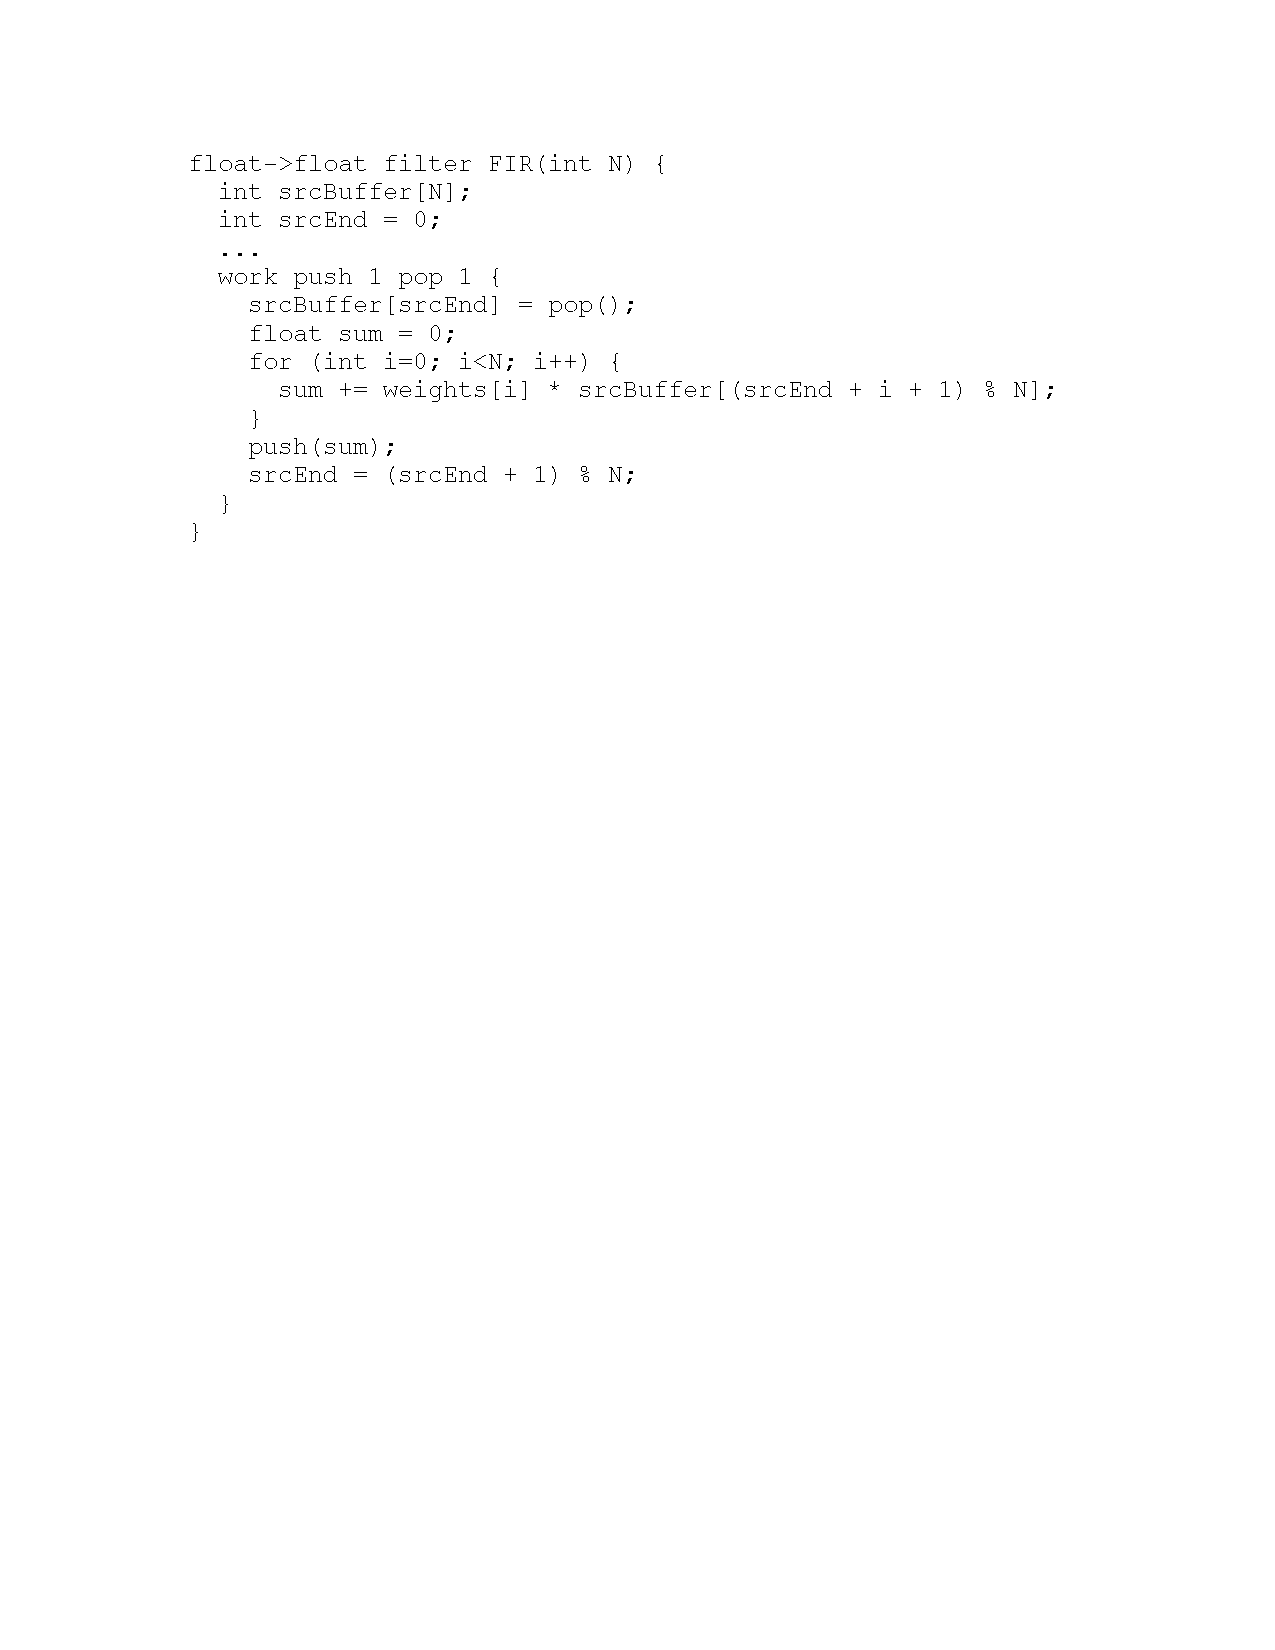
\includegraphics[width=3.3in]{figures/fir-nopeeking.pdf}\label{fig:fir-nopeeking}}
\subfigure[]{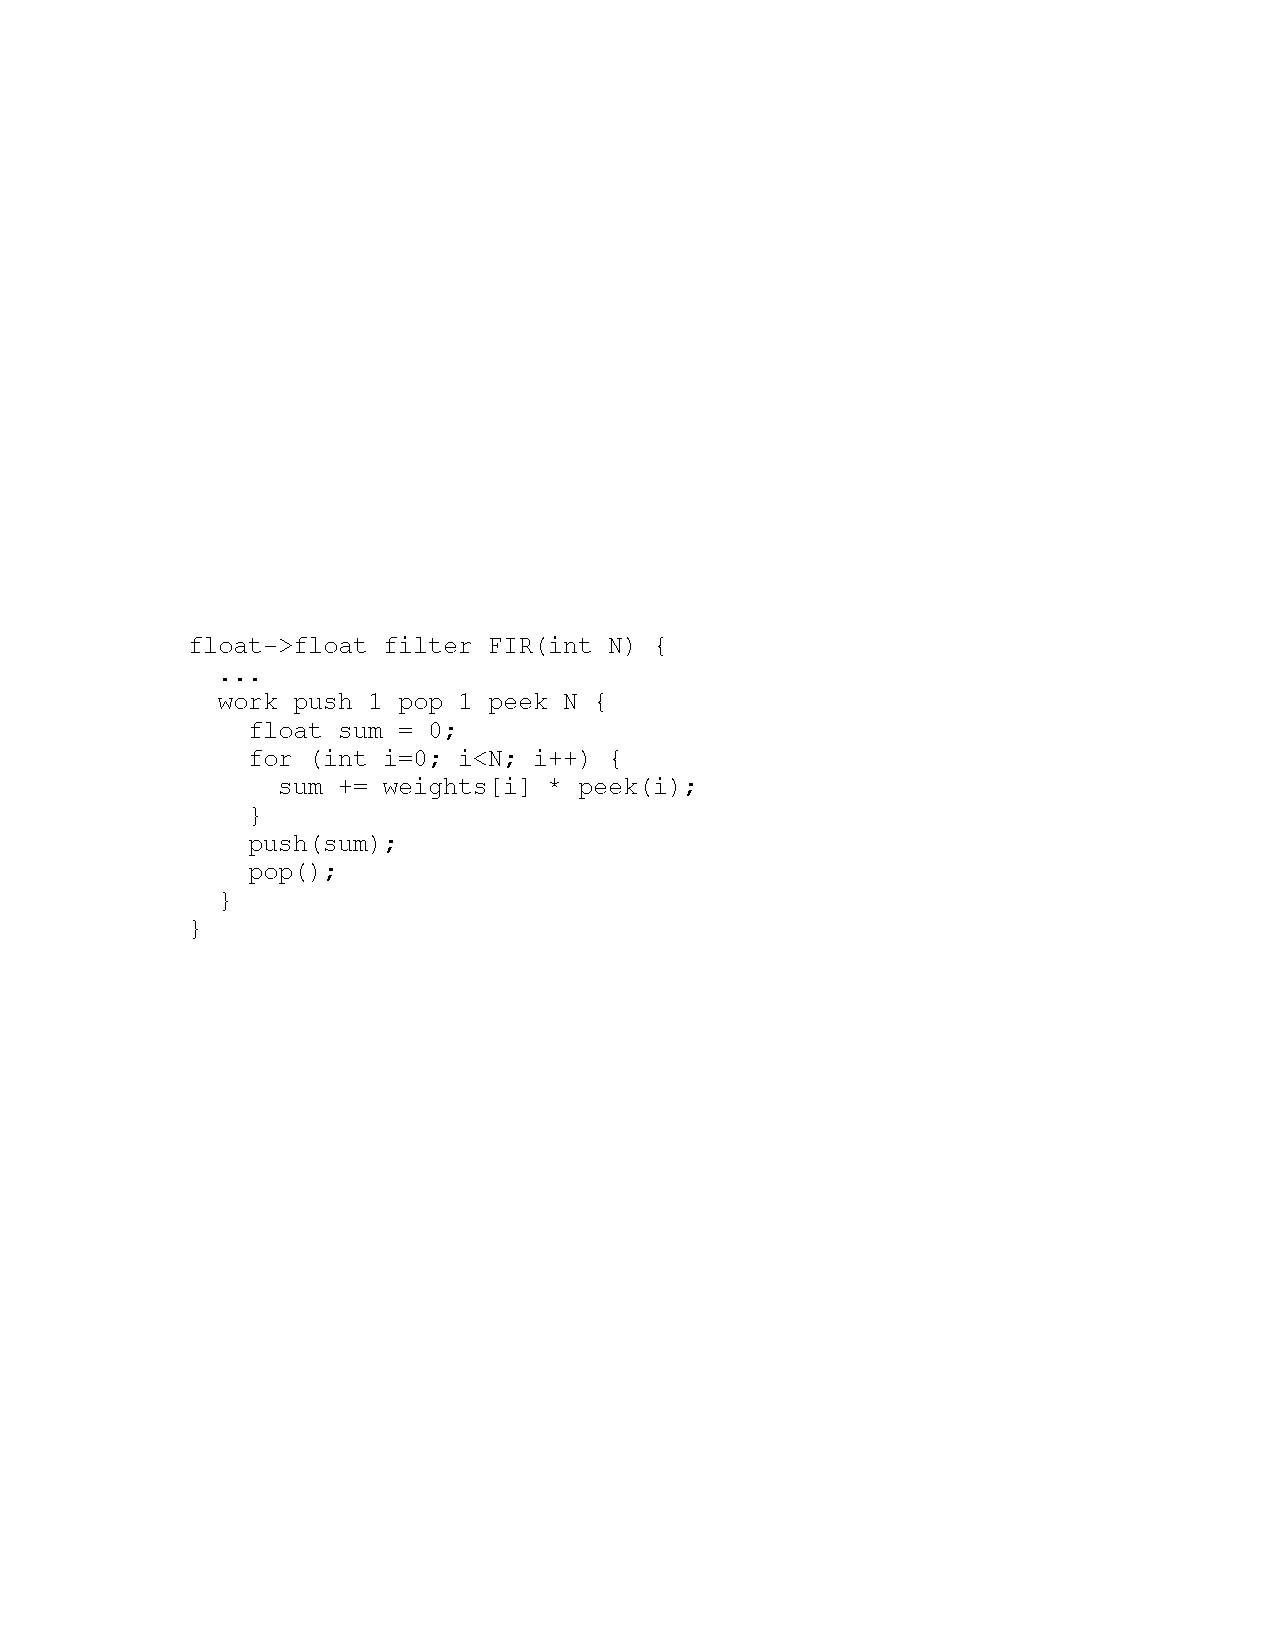
\includegraphics[width=3.3in]{figures/fir-peeking.pdf}\label{fig:fir-peeking}}
\caption[Two implementations of an FIR filter.]{\label{fig:fir-code}
  Two StreamIt implementations of an FIR filter:
   (a) the non-peeking version implemented via a
  stateful circular buffer; and (b) the peeking version. Only steady-state implementation is
  given.}
\end{figure}

The framework presented is defined on a model of computation that is
agnostic of source language.  To evaluate our techniques we have
implemented them in the context of the StreamIt compiler
infrastructure~\cite{gordon-asplos06}.  Our transformations are guided
by the parallelization management techniques presented
in~\cite{gordon-asplos06}.  We employ 3 real-world benchmarks from the
StreamIt Benchmark Suite~\cite{streamit-suite} that include sliding
window computation.  We demonstrate the effectiveness of our
techniques by comparing them to previously published techniques on 2
multicore architectures: a 16-core SMP shared-memory multicore and the
64-core distributed-memory Tilera TILE64.  We show that
our techniques are required to achieve scalable parallelization on
both architectures, achieving a 6.7x mean speedup on the 16-core SMP
and a 1.8x mean speedup on the 64-core distributed memory multicore
over a previously published technique.

\subsection{Contributions}
This paper makes the following contributions:
\begin{itemize}
  % \myitem{Motivation for Exposing Sliding Windows in Stream
  %   Languages}: Without exposing sliding windows in the language, it
  % requires heroic effort by the compiler to analyze the access patterns
  % of such a filter. Without success, the compiler will not be able to
  % data-parallelize these filters.  This will prevent robust 
  % parallelization scalability for streaming applications.

  \myitem{Generalized Fission of Sliding Window Filters}: We present a
  transformation that fisses sliding window filters with multiple
  input and multiple outputs.  The technique also supports filters
  that with multiple schedules of execution.  General fission defines
  a precise pattern of communication of input data to the products
  that can be reasoned upon by our other techniques.

  \myitem{Sharing Reduction}: We are the first to present a technique
  that decides when it is possible to decrease the amount of sharing
  between fission products by altering the steady-state of a stream
  graph, thus decreasing inter-core communication.  The technique
  reasons about all the sliding window filters of the stream graph,
  and when possible, reduces the sharing requirement to below a given
  threshold percent of the total input of the filters. 

  \myitem{Data Parallelization of Stream Graph}: We present a
  framework for data-parallelizing all of the filters of a stream
  graph employing the fission transformation on individual filters and
  applying sharing reduction when possible.  This framework optimizes
  for spatial locality and enables the compiler to automatically and
  effectively manage parallelization across varying multicore
  architectures.

  \myitem{Enable Robust Parallelization Scaling for Multicores}: For
  streaming applications with sliding window computation, previously
  published data-parallelization transformations do not scale for our
  target multicores. Our techniques enable robust parallelization
  scalability by reducing inter-core communication.  We achieve a 17x
  mean parallelization speedup for a 16-core SMP and a 62.3x mean
  parallelization speedup for the 64-core TILE64 across our benchmarks.

\end{itemize}

% \begin{figure}[t]
% \centering
% \begin{subfloat}
% \begin{minipage}[b]{0.45\textwidth}
% \eightpoint
% \begin{verbatim}
% float->float filter FIR(int N) {
%   int srcBuffer[N];
%   int srcEnd = 0; 
%   ...
%   work push 1 pop 1 {
%     srcBuffer[srcEnd] = pop();
%     float sum = 0;
%     for (int i=0; i<N; i++) {
%       sum += weights[i] * srcBuffer[(srcEnd + i + 1) % N];
%     }
%     push(sum);
%     srcEnd = (srcEnd + 1) % N;
%   }
% }
% \end{verbatim}
% \vspace{-8pt}
% \end{minipage}%
% \caption{ \label{fig:fir-nopeeking}}
% \end{subfloat}%
% \qquad
% \begin{subfloat}
% \begin{minipage}[b]{0.45\textwidth}
% \eightpoint
% \begin{verbatim}
% float->float filter FIR(int N) {
%   ...
%   work push 1 pop 1 peek N {
%     float sum = 0;
%     for (int i=0; i<N; i++) {
%       sum += weights[i] * peek(i);
%     }
%     push(sum);
%     pop();
%   }
% }
% \end{verbatim}
% \vspace{-18pt}
% \end{minipage}
% \caption{ \label{fig:fir-streamit}}
% \end{subfloat}
% \caption[Two implementations of an FIR filter.]{\label{fig:fir-code}
%   Two StreamIt implementations of an FIR filter:
%    \subref{fig:fir-nopeeking} the non-peeking version implemented via a
%   stateful circular buffer; and \subref{fig:fir-streamit} the peeking version. Only steady-state implementation is
%   given.}
% \end{figure}
